\documentclass{article} % For LaTeX2e
\usepackage{graphicx}
\usepackage{amssymb}
\usepackage{amsmath}
%\usepackage{nips14submit_e,times}
\usepackage{hyperref}
\usepackage{url}
\usepackage{natbib}
\usepackage{subcaption}

\usepackage[margin=1.5in]{geometry}
%\documentstyle[nips14submit_09,times,art10]{article} % For LaTeX 2.09
\let\polishl\l
\DeclareMathOperator{\x}{\mathbf{x}}
\DeclareMathOperator{\e}{\mathbf{e}}
\DeclareMathOperator{\M}{\mathbf{M}}
\DeclareMathOperator{\w}{\mathbf{w}}
\newcommand{\fix}{\marginpar{FIX}}
\newcommand{\new}{\marginpar{NEW}}
\edef\polishl{\l} 



\RequirePackage{latexsym}
\RequirePackage{amsmath}
\RequirePackage{amssymb} 
\RequirePackage{color} 
\RequirePackage{bm}
\RequirePackage{color}
\RequirePackage{picinpar}

%%%%%%%% Stock standard definitions %%%%%%%%%%%%%%%

\newcommand{\wbt}{\widetilde{\mathbf{w}}}
\DeclareMathOperator{\ab}{\mathbf{a}}
\DeclareMathOperator{\abh}{\widehat{\ab}}
\DeclareMathOperator{\bb}{\mathbf{b}}
\DeclareMathOperator{\bbh}{\widehat{\bb}}
\DeclareMathOperator{\cb}{\mathbf{c}}
\DeclareMathOperator{\db}{\mathbf{d}}
\DeclareMathOperator{\eb}{\mathbf{e}}
\DeclareMathOperator{\fb}{\mathbf{f}}
\DeclareMathOperator{\gb}{\mathbf{g}}
\DeclareMathOperator{\hb}{\mathbf{h}}
\DeclareMathOperator{\ib}{\mathbf{i}}
\DeclareMathOperator{\jb}{\mathbf{j}}
\DeclareMathOperator{\kb}{\mathbf{k}}
\DeclareMathOperator{\lb}{\mathbf{l}}
\DeclareMathOperator{\mb}{\mathbf{m}}
\DeclareMathOperator{\nbb}{\mathbf{n}}
\DeclareMathOperator{\ob}{\mathbf{o}}
\DeclareMathOperator{\pb}{\mathbf{p}}
\DeclareMathOperator{\qb}{\mathbf{q}}
\DeclareMathOperator{\rb}{\mathbf{r}}
\DeclareMathOperator{\sbb}{\mathbf{s}}
\DeclareMathOperator{\tb}{\mathbf{t}}
\DeclareMathOperator{\ub}{\mathbf{u}}
\DeclareMathOperator{\vb}{\mathbf{v}}
\DeclareMathOperator{\wb}{\mathbf{w}}
\DeclareMathOperator{\xb}{\mathbf{x}}
\DeclareMathOperator{\yb}{\mathbf{y}}
\DeclareMathOperator{\zb}{\mathbf{z}}
\renewcommand{\l}{\ell}

\DeclareMathOperator{\atilde}{\tilde{\ab}}
\DeclareMathOperator{\btilde}{\tilde{\bb}}
\DeclareMathOperator{\ctilde}{\tilde{\cb}}
\DeclareMathOperator{\dtilde}{\tilde{\db}}
\DeclareMathOperator{\etilde}{\tilde{\eb}}
\DeclareMathOperator{\ftilde}{\tilde{\fb}}
\DeclareMathOperator{\gtilde}{\tilde{\gb}}
\DeclareMathOperator{\htilde}{\tilde{\hb}}
\DeclareMathOperator{\itilde}{\tilde{\ib}}
\DeclareMathOperator{\jtilde}{\tilde{\jb}}
\DeclareMathOperator{\ktilde}{\tilde{\kb}}
\DeclareMathOperator{\ltilde}{\tilde{\lb}}
\DeclareMathOperator{\mtilde}{\tilde{\mb}}
\DeclareMathOperator{\ntilde}{\tilde{\nbb}}
\DeclareMathOperator{\otilde}{\tilde{\ob}}
\DeclareMathOperator{\ptilde}{\tilde{\pb}}
\DeclareMathOperator{\qtilde}{\tilde{\qb}}
\DeclareMathOperator{\rtilde}{\tilde{\rb}}
\DeclareMathOperator{\stilde}{\tilde{\sbb}}
\DeclareMathOperator{\ttilde}{\tilde{\tb}}
\DeclareMathOperator{\utilde}{\tilde{\ub}}
\DeclareMathOperator{\vtilde}{\tilde{\vb}}
\DeclareMathOperator{\wtilde}{\tilde{\wb}}
\DeclareMathOperator{\xtilde}{\tilde{\xb}}
\DeclareMathOperator{\ytilde}{\tilde{\yb}}
\DeclareMathOperator{\ztilde}{\tilde{\zb}}

\DeclareMathOperator{\abar}{\bar{\ab}}
\DeclareMathOperator{\bbar}{\bar{\bb}}
\DeclareMathOperator{\cbar}{\bar{\cb}}
\DeclareMathOperator{\dbar}{\bar{\db}}
\DeclareMathOperator{\ebar}{\bar{\eb}}
\DeclareMathOperator{\fbar}{\bar{\fb}}
\DeclareMathOperator{\gbar}{\bar{\gb}}
\DeclareMathOperator{\hbbar}{\bar{\hb}}
\DeclareMathOperator{\ibar}{\bar{\ib}}
\DeclareMathOperator{\jbar}{\bar{\jb}}
\DeclareMathOperator{\kbar}{\bar{\kb}}
\DeclareMathOperator{\lbar}{\bar{\lb}}
\DeclareMathOperator{\mbar}{\bar{\mb}}
\DeclareMathOperator{\nbar}{\bar{\nbb}}
\DeclareMathOperator{\obar}{\bar{\ob}}
\DeclareMathOperator{\pbar}{\bar{\pb}}
\DeclareMathOperator{\qbar}{\bar{\qb}}
\DeclareMathOperator{\rbar}{\bar{\rb}}
\DeclareMathOperator{\sbar}{\bar{\sbb}}
\DeclareMathOperator{\tbar}{\bar{\tb}}
\DeclareMathOperator{\ubar}{\bar{\ub}}
\DeclareMathOperator{\vbar}{\bar{\vb}}
\DeclareMathOperator{\wbar}{\bar{\wb}}
\DeclareMathOperator{\xbar}{\bar{\xb}}
\DeclareMathOperator{\ybar}{\bar{\yb}}
\DeclareMathOperator{\zbar}{\bar{\zb}}

\DeclareMathOperator{\Ab}{\mathbf{A}}
\DeclareMathOperator{\Bb}{\mathbf{B}}
\DeclareMathOperator{\Cb}{\mathbf{C}}
\DeclareMathOperator{\Db}{\mathbf{D}}
\DeclareMathOperator{\Eb}{\mathbf{E}}
\DeclareMathOperator{\Fb}{\mathbf{F}}
\DeclareMathOperator{\Gb}{\mathbf{G}}
\DeclareMathOperator{\Hb}{\mathbf{H}}
\DeclareMathOperator{\Ib}{\mathbf{I}}
\DeclareMathOperator{\Jb}{\mathbf{J}}
\DeclareMathOperator{\Kb}{\mathbf{K}}
\DeclareMathOperator{\Lb}{\mathbf{L}}
\DeclareMathOperator{\Mb}{\mathbf{M}}
\DeclareMathOperator{\Nb}{\mathbf{N}}
\DeclareMathOperator{\Ob}{\mathbf{O}}
\DeclareMathOperator{\Pb}{\mathbf{P}}
\DeclareMathOperator{\Qb}{\mathbf{Q}}
\DeclareMathOperator{\Rb}{\mathbf{R}}
\DeclareMathOperator{\Sbb}{\mathbf{S}}
\DeclareMathOperator{\Tb}{\mathbf{T}}
\DeclareMathOperator{\Ub}{\mathbf{U}}
\DeclareMathOperator{\Vb}{\mathbf{V}}
\DeclareMathOperator{\Wb}{\mathbf{W}}
\DeclareMathOperator{\Xb}{\mathbf{X}}
\DeclareMathOperator{\Xbt}{\widetilde{\Xb}}
\DeclareMathOperator{\Xbh}{\widehat{\Xb}}
\DeclareMathOperator{\Xbs}{\widetilde{\Xb}}
\DeclareMathOperator{\Zbs}{\widetilde{\Zb}}
\DeclareMathOperator{\Kbs}{\widetilde{\Kb}}
\DeclareMathOperator{\Zbh}{\widehat{\Zb}}
\DeclareMathOperator{\Ubh}{\widehat{\Ub}}
\DeclareMathOperator{\Yb}{\mathbf{Y}}
\DeclareMathOperator{\Zb}{\mathbf{Z}}

\DeclareMathOperator{\Abar}{\bar{A}}
\DeclareMathOperator{\Bbar}{\bar{B}}
\DeclareMathOperator{\Cbar}{\bar{C}}
\DeclareMathOperator{\Dbar}{\bar{D}}
\DeclareMathOperator{\Ebar}{\bar{E}}
\DeclareMathOperator{\Fbar}{\bar{F}}
\DeclareMathOperator{\Gbar}{\bar{G}}
\DeclareMathOperator{\Hbar}{\bar{H}}
\DeclareMathOperator{\Ibar}{\bar{I}}
\DeclareMathOperator{\Jbar}{\bar{J}}
\DeclareMathOperator{\Kbar}{\bar{K}}
\DeclareMathOperator{\Lbar}{\bar{L}}
\DeclareMathOperator{\Mbar}{\bar{M}}
\DeclareMathOperator{\Nbar}{\bar{N}}
\DeclareMathOperator{\Obar}{\bar{O}}
\DeclareMathOperator{\Pbar}{\bar{P}}
\DeclareMathOperator{\Qbar}{\bar{Q}}
\DeclareMathOperator{\Rbar}{\bar{R}}
\DeclareMathOperator{\Sbar}{\bar{S}}
\DeclareMathOperator{\Tbar}{\bar{T}}
\DeclareMathOperator{\Ubar}{\bar{U}}
\DeclareMathOperator{\Vbar}{\bar{V}}
\DeclareMathOperator{\Wbar}{\bar{W}}
\DeclareMathOperator{\Xbar}{\bar{X}}
\DeclareMathOperator{\Ybar}{\bar{Y}}
\DeclareMathOperator{\Zbar}{\bar{Z}}

\DeclareMathOperator{\Abbar}{\bar{\Ab}}
\DeclareMathOperator{\Bbbar}{\bar{\Bb}}
\DeclareMathOperator{\Cbbar}{\bar{\Cb}}
\DeclareMathOperator{\Dbbar}{\bar{\Db}}
\DeclareMathOperator{\Ebbar}{\bar{\Eb}}
\DeclareMathOperator{\Fbbar}{\bar{\Fb}}
\DeclareMathOperator{\Gbbar}{\bar{\Gb}}
\DeclareMathOperator{\Hbbar}{\bar{\Hb}}
\DeclareMathOperator{\Ibbar}{\bar{\Ib}}
\DeclareMathOperator{\Jbbar}{\bar{\Jb}}
\DeclareMathOperator{\Kbbar}{\bar{\Kb}}
\DeclareMathOperator{\Lbbar}{\bar{\Lb}}
\DeclareMathOperator{\Mbbar}{\bar{\Mb}}
\DeclareMathOperator{\Nbbar}{\bar{\Nb}}
\DeclareMathOperator{\Obbar}{\bar{\Ob}}
\DeclareMathOperator{\Pbbar}{\bar{\Pb}}
\DeclareMathOperator{\Qbbar}{\bar{\Qb}}
\DeclareMathOperator{\Rbbar}{\bar{\Rb}}
\DeclareMathOperator{\Sbbar}{\bar{\Sb}}
\DeclareMathOperator{\Tbbar}{\bar{\Tb}}
\DeclareMathOperator{\Ubbar}{\bar{\Ub}}
\DeclareMathOperator{\Vbbar}{\bar{\Vb}}
\DeclareMathOperator{\Wbbar}{\bar{\Wb}}
\DeclareMathOperator{\Xbbar}{\bar{\Xb}}
\DeclareMathOperator{\Ybbar}{\bar{\Yb}}
\DeclareMathOperator{\Zbbar}{\bar{\Zb}}

\DeclareMathOperator{\Ahat}{\widehat{A}}
\DeclareMathOperator{\Bhat}{\widehat{B}}
\DeclareMathOperator{\Chat}{\widehat{C}}
\DeclareMathOperator{\Dhat}{\widehat{D}}
\DeclareMathOperator{\Ehat}{\widehat{E}}
\DeclareMathOperator{\Fhat}{\widehat{F}}
\DeclareMathOperator{\Ghat}{\widehat{G}}
\DeclareMathOperator{\Hhat}{\widehat{H}}
\DeclareMathOperator{\Ihat}{\widehat{I}}
\DeclareMathOperator{\Jhat}{\widehat{J}}
\DeclareMathOperator{\Khat}{\widehat{K}}
\DeclareMathOperator{\Lhat}{\widehat{L}}
\DeclareMathOperator{\Mhat}{\widehat{M}}
\DeclareMathOperator{\Nhat}{\widehat{N}}
\DeclareMathOperator{\Ohat}{\widehat{O}}
\DeclareMathOperator{\Phat}{\widehat{P}}
\DeclareMathOperator{\Qhat}{\widehat{Q}}
\DeclareMathOperator{\Rhat}{\widehat{R}}
\DeclareMathOperator{\Shat}{\widehat{S}}
\DeclareMathOperator{\That}{\widehat{T}}
\DeclareMathOperator{\Uhat}{\widehat{U}}
\DeclareMathOperator{\Vhat}{\widehat{V}}
\DeclareMathOperator{\What}{\widehat{W}}
\DeclareMathOperator{\Xhat}{\widehat{X}}
\DeclareMathOperator{\Yhat}{\widehat{Y}}
\DeclareMathOperator{\Zhat}{\widehat{Z}}

\DeclareMathOperator{\Abhat}{\widehat{\Ab}}
\DeclareMathOperator{\Bbhat}{\widehat{\Bb}}
\DeclareMathOperator{\Cbhat}{\widehat{\Cb}}
\DeclareMathOperator{\Dbhat}{\widehat{\Db}}
\DeclareMathOperator{\Ebhat}{\widehat{\Eb}}
\DeclareMathOperator{\Fbhat}{\widehat{\Fb}}
\DeclareMathOperator{\Gbhat}{\widehat{\Gb}}
\DeclareMathOperator{\Hbhat}{\widehat{\Hb}}
\DeclareMathOperator{\Ibhat}{\widehat{\Ib}}
\DeclareMathOperator{\Jbhat}{\widehat{\Jb}}
\DeclareMathOperator{\Kbhat}{\widehat{\Kb}}
\DeclareMathOperator{\Lbhat}{\widehat{\Lb}}
\DeclareMathOperator{\Mbhat}{\widehat{\Mb}}
\DeclareMathOperator{\Nbhat}{\widehat{\Nb}}
\DeclareMathOperator{\Obhat}{\widehat{\Ob}}
\DeclareMathOperator{\Pbhat}{\widehat{\Pb}}
\DeclareMathOperator{\Qbhat}{\widehat{\Qb}}
\DeclareMathOperator{\Rbhat}{\widehat{\Rb}}
\DeclareMathOperator{\Sbhat}{\widehat{\Sb}}
\DeclareMathOperator{\Tbhat}{\widehat{\Tb}}
\DeclareMathOperator{\Ubhat}{\widehat{\Ub}}
\DeclareMathOperator{\Vbhat}{\widehat{\Vb}}
\DeclareMathOperator{\Wbhat}{\widehat{\Wb}}
\DeclareMathOperator{\Xbhat}{\widehat{\Xb}}
\DeclareMathOperator{\Ybhat}{\widehat{\Yb}}
\DeclareMathOperator{\Zbhat}{\widehat{\Zb}}

\DeclareMathOperator{\Acal}{\mathcal{A}}
\DeclareMathOperator{\Bcal}{\mathcal{B}}
\DeclareMathOperator{\Ccal}{\mathcal{C}}
\DeclareMathOperator{\Dcal}{\mathcal{D}}
\DeclareMathOperator{\Ecal}{\mathcal{E}}
\DeclareMathOperator{\Fcal}{\mathcal{F}}
\DeclareMathOperator{\Gcal}{\mathcal{G}}
\DeclareMathOperator{\Hcal}{\mathcal{H}}
\DeclareMathOperator{\Ical}{\mathcal{I}}
\DeclareMathOperator{\Jcal}{\mathcal{J}}
\DeclareMathOperator{\Kcal}{\mathcal{K}}
\DeclareMathOperator{\Lcal}{\mathcal{L}}
\DeclareMathOperator{\Mcal}{\mathcal{M}}
\DeclareMathOperator{\Ncal}{\mathcal{N}}
\DeclareMathOperator{\Ocal}{\mathcal{O}}
\DeclareMathOperator{\Pcal}{\mathcal{P}}
\DeclareMathOperator{\Qcal}{\mathcal{Q}}
\DeclareMathOperator{\Rcal}{\mathcal{R}}
\DeclareMathOperator{\Scal}{\mathcal{S}}
\DeclareMathOperator{\Scalt}{\widetilde{\Scal}}
\DeclareMathOperator{\Tcal}{\mathcal{T}}
\DeclareMathOperator{\Ucal}{\mathcal{U}}
\DeclareMathOperator{\Vcal}{\mathcal{V}}
\DeclareMathOperator{\Wcal}{\mathcal{W}}
\DeclareMathOperator{\Xcal}{\mathcal{X}}
\DeclareMathOperator{\Ycal}{\mathcal{Y}}
\DeclareMathOperator{\Zcal}{\mathcal{Z}}

\DeclareMathOperator{\Atilde}{\widetilde{A}}
\DeclareMathOperator{\Btilde}{\widetilde{B}}
\DeclareMathOperator{\Ctilde}{\widetilde{C}}
\DeclareMathOperator{\Dtilde}{\widetilde{D}}
\DeclareMathOperator{\Etilde}{\widetilde{E}}
\DeclareMathOperator{\Ftilde}{\widetilde{F}}
\DeclareMathOperator{\Gtilde}{\widetilde{G}}
\DeclareMathOperator{\Htilde}{\widetilde{H}}
\DeclareMathOperator{\Itilde}{\widetilde{I}}
\DeclareMathOperator{\Jtilde}{\widetilde{J}}
\DeclareMathOperator{\Ktilde}{\widetilde{K}}
\DeclareMathOperator{\Ltilde}{\widetilde{L}}
\DeclareMathOperator{\Mtilde}{\widetilde{M}}
\DeclareMathOperator{\Ntilde}{\widetilde{N}}
\DeclareMathOperator{\Otilde}{\widetilde{O}}
\DeclareMathOperator{\Ptilde}{\widetilde{P}}
\DeclareMathOperator{\Qtilde}{\widetilde{Q}}
\DeclareMathOperator{\Rtilde}{\widetilde{R}}
\DeclareMathOperator{\Stilde}{\widetilde{S}}
\DeclareMathOperator{\Ttilde}{\widetilde{T}}
\DeclareMathOperator{\Utilde}{\widetilde{U}}
\DeclareMathOperator{\Vtilde}{\widetilde{V}}
\DeclareMathOperator{\Wtilde}{\widetilde{W}}
\DeclareMathOperator{\Xtilde}{\widetilde{X}}
\DeclareMathOperator{\Ytilde}{\widetilde{Y}}
\DeclareMathOperator{\Ztilde}{\widetilde{Z}}


%%%%%%%% Widely accepted definitions %%%%%%%%%%%%%%%

\DeclareMathOperator{\CC}{\mathbb{C}} % Complex numbers
\DeclareMathOperator{\EE}{\mathbb{E}} % Expectation
\DeclareMathOperator{\KK}{\mathbb{K}} % Arbitrary field
\DeclareMathOperator{\MM}{\mathbb{M}} % Median
\DeclareMathOperator{\NN}{\mathbb{N}} % Natural numbers
\DeclareMathOperator{\PP}{\mathbb{P}} % Probability
\DeclareMathOperator{\QQ}{\mathbb{Q}} % Rationals
\DeclareMathOperator{\RR}{\mathbb{R}} % Real numbers 
\DeclareMathOperator{\ZZ}{\mathbb{Z}} % Integers

\DeclareMathOperator{\one}{\mathbf{1}}  % Identity
\DeclareMathOperator{\zero}{\mathbf{0}} % Zero
\DeclareMathOperator{\TRUE}{\mathbf{TRUE}}  % True
\DeclareMathOperator{\FALSE}{\mathbf{FALSE}}  % False

\DeclareMathOperator*{\mini}{\mathop{\mathrm{minimize}}}
\DeclareMathOperator*{\maxi}{\mathop{\mathrm{maximize}}}
\DeclareMathOperator*{\argmin}{\mathop{\mathrm{argmin}}}
\DeclareMathOperator*{\argmax}{\mathop{\mathrm{argmax}}}
\DeclareMathOperator*{\argsup}{\mathop{\mathrm{argsup}}}
\DeclareMathOperator*{\arginf}{\mathop{\mathrm{arginf}}}
\DeclareMathOperator{\sgn}{\mathop{\mathrm{sign}}}
\DeclareMathOperator{\sign}{\mathop{\mathrm{sign}}}
\DeclareMathOperator{\tr}{\mathop{\mathrm{tr}}}
\DeclareMathOperator{\rank}{\mathop{\mathrm{rank}}}
\DeclareMathOperator{\traj}{\mathop{\mathrm{Traj}}}

%%%%%%%% Bold Greek Letters %%%%%%%%%%%%%%%
\DeclareMathOperator{\sigmab}{\bm{\sigma}}
\DeclareMathOperator{\Sigmab}{\mathbf{\Sigma}}


%%%%%%%% Mess around with LaTeX %%%%%%%%%%%%%%%

%% Some style files might actually define these variables.
%% So don't mess with them if they are already defined

\ifx\BlackBox\undefined
\newcommand{\BlackBox}{\rule{1.5ex}{1.5ex}}  % end of proof
\fi

\ifx\proof\undefined
\newenvironment{proof}{\par\noindent{\bf Proof\ }}{\hfill\BlackBox\\[2mm]}
% \else
% \renewenvironment{proof}{\par\noindent{\bf Proof\ }}{\hfill\BlackBox\\[2mm]}
\fi

%Trying to put all on Section track
%\makeatletter
%\@addtoreset{equation}{section}
%\def\theequation{\thesection.\arabic{equation}}
%\def\thetheorem{\thesection.\arabic{theorem}}
%\makeatother

%the below clashes with the previous defs of them... 
%in the style files
%\newtheorem{theorem}{Theorem}[section]
%\newtheorem{lemma}[theorem]{Lemma}
%\newtheorem{corollary}[theorem]{Corollary}
%\newtheorem{conjecture}[conjecture]{Conjecture}


%%%%%%%% Utility functions %%%%%%%%%%%%%%%

\newcommand{\eq}[1]{(\ref{#1})} 
\newcommand{\mymatrix}[2]{\left[\begin{array}{#1} #2 \end{array}\right]}
\newcommand{\mychoose}[2]{\left(\begin{array}{c} #1 \\ #2 \end{array}\right)}
\newcommand{\mydet}[1]{\det\left[ #1 \right]}
\newcommand{\sembrack}[1]{[\![#1]\!]}

\newcommand{\ea}{\emph{et al. }}
\newcommand{\eg}{\emph{e.g. }}
\newcommand{\ie}{\emph{i.e., }}

\newcommand{\mnote}[1]{\marginpar{#1}}
\newcommand{\note}[1]{{\bf {#1}}}

%%%%%%%% Specific symbols for this project %%%%%%%%%%%%%%%

\DeclareMathOperator{\half}{\frac{1}{2}}

\newcommand{\Ref}[1]{\hfill\Green{[#1]}}
\DeclareMathOperator{\XX}{\mathcal{X}}
\newcommand{\ar}{\implies}
\newcommand{\yh}{\hat{y}}
\DeclareMathOperator{\lan}{\langle}
\DeclareMathOperator{\ran}{\rangle}

\DeclareMathOperator{\dc}{\mathrm{dc}}

\DeclareMathOperator{\Utb}{\widetilde{\Ub}}
\DeclareMathOperator{\Stb}{\widetilde{\Sbb}}

\ifx\Brown\undefined
\definecolor{brown}{rgb}{0.5,0.1,0.1}
\newcommand{\Brown}[1]{\color{brown}{#1}\color{black}}
\fi

\ifx\Red\undefined
\definecolor{red}{rgb}{1.0,0,0}
\newcommand{\Red}[1]{\color{red}{#1}\color{black}}
\fi

\ifx\Green\undefined
\definecolor{green}{rgb}{0,0.4,0}
\newcommand{\Green}[1]{\color{green}{#1}\color{black}}
\fi

\ifx\Blue\undefined
\definecolor{blue}{rgb}{0,0,1.0}
\newcommand{\Blue}[1]{\color{blue}{#1}\color{black}}
\fi



\newcommand{\beq}{\begin{equation}}
\newcommand{\eeq}{\end{equation}}
\newcommand{\beh}{\begin{conjecture}}
\newcommand{\eeh}{\end{conjecture}}
\newcommand\bel{\begin{lemma}}
\newcommand\eel{\end{lemma}}
\newcommand\bet{\begin{theoreme}}
\newcommand\eet{\end{theoreme}}
\newcommand\bex{\begin{example}}
\newcommand\eex{\end{example}}
\newcommand\bed{\begin{definition}}
\newcommand\eed{\end{definition}}
\newcommand\bep{\begin{proposition}}
\newcommand\eep{\end{proposition}}
\newcommand\ber{\begin{remark}}
\newcommand\eer{\end{remark}}
\newcommand\bec{\begin{corollary}}
\newcommand\eec{\end{corollary}}
%\newcommand\proof{\noindent {\bf Proof.}\ \ }
\newcommand\qed{\hfill$\Box$\medskip}
\newcommand\cP{{\mathcal P}}
\newcommand\cJ{{\mathcal J}}
\newcommand\cD{{\mathcal D}}
\newcommand\cC{{\mathcal C}}
\newcommand\cO{{\mathcal O}}
\newcommand\cS{{\mathcal S}}
\newcommand\cT{{\mathcal T}}
\newcommand\cV{{\mathcal V}}
\newcommand\cW{{\mathcal W}}
\newcommand\cY{{\mathcal Y}}
\newcommand\cF{{\mathcal F}}
\newcommand\cU{{\mathcal U}}
\newcommand\cE{{\mathcal E}}
\newcommand\cG{{\mathcal G}}
\newcommand\cB{{\mathcal B}}
\newcommand\cI{{\rm I}}
\newcommand\cN{{\mathcal N}}
\newcommand\cM{{\mathcal M}}
\newcommand\cA{{\mathcal A}}
\newcommand\cQ{{\mathcal Q}}
\newcommand\cK{{\mathcal K}}
\newcommand\cZ{{\mathcal Z}}
\newcommand\CAP{{\rm cap}}
\newcommand\ENT{{\rm ent}}
\newcommand\gr{{\rm gr}}

\def\qq{{\mathbb Q}}
\def\ff{{\mathbb F}}
\def\rr{{\mathbb R}}
\def\zz{{\mathbb Z}}
\def\cc{{\mathbb C}}
\def\nn{{\mathbb N}}
\def\kk{{\mathbb K}}
\def\ee{{\mathbb E}}
\def\ww{{\mathbb W}}
\def\hh{{\mathbb H}}
\def\ss{{\mathbb S}}
\def\tt{{\mathbb T}}
\def\pp{{\mathbb P}}



\newtheorem{theoreme}{Theorem} %[section]
\newtheorem{proposition}[theoreme]{Proposition}
\newtheorem{lemma}[theoreme]{Lemma}
\newtheorem{definition}[theoreme]{Definition}
\newtheorem{corollary}[theoreme]{Corollary}
\newtheorem{remark}[theoreme]{Remark}
\newtheorem{example}[theoreme]{Example}
\newtheorem{examples}[theoreme]{Examples}
%\newtheorem{conjecture}[theoreme]{Conjecture}
\newtheorem{conjecture}{Conjecture}

\title{A Theory of Diversity}

\author{Micha{\polishl} Derezi\'{n}ski}

\date{CMPS 290 Final Report, Fall 2014}
% \author{
% Micha{\l } Derezi\'{n}ski\\
% Computer Science Department\\
% University of California, Santa Cruz\\
% CA 95064, U.S.A.\\
% \texttt{mderezin@soe.ucsc.edu}
% }



\begin{document}


\maketitle

\section{Population Diversity}
\label{sec:population-diversity}
The notion of diversity has been analyzed for various settings and
disciplines. Many different definitions have been proposed, among
which Shannon entropy could be considered as the most standard and widely
accepted. We will first discuss this definition in a simple setting of
measuring population diversity. Consider an arbitrary finite set $S$ of
objects, where each has a label assigned to it from set $T$ by a function
$f:S\rightarrow T$. We want to measure the diversity of set $S$ with
respect to the label assignment. It is clear, that having no other
information about the objects in $S$, the sufficient statistic here
would be a function $N:T\rightarrow \nn$, that for each label produces
the number of elements in $S$ that have been assigned it. We can
further separate this information into the size of $S$ and the
probability distribution $P_S$ over the labels, when drawing a random
element from $S$. We can use this distribution to observe what kind of
label biases are present in the population $S$. Shannon entropy
$H(P_S)$ measures the amount of uncertainty in $P_S$ - the more
balanced the distribution, the more uncertainty 
is maintained. Notice, that the uniform distribution is favored here as
the most diverse, balanced and having no inherent biases. However, is
it always the case that the uniform distribution should have those
properties? 

Consider a hypothetical civilization divided into countries, where a
new land has been discovered and colonized by a small group of
independent settlers. Then, the land is further populated through
immigration from other countries. Due to some political reasons, the
settlers are much more inclined to accept immigrants from country $A$
than from country $B$. In other words, there is an inherent bias in
the population against country $B$, and in favor of country
$A$. However, given that scenario, it is still entirely possible that
the distribution of immigrants (with respect to their country of
origin) would end up perfectly uniform, by the simple fact that there
could be more potential immigrants applying from $B$ than from $A$. In
this case, observing the population from within would suggest that it
is perfectly diverse and free of biases, contrary to what we know
looking at the bigger picture. 

The key factor in the above example is that we measure the diversity
of a population in context of a larger universe, that itself has a
certain distribution of labels, which may not be uniform.
To formalize this, we will propose
a generative population model that incorporates this concept of
a context distribution. Suppose we want to measure the diversity
of a population $S$ within a larger universe $U$ of objects with
labels assigned from the set $T$. We will assume that $S$ was
generated from 
$U$ as follows: We draw an element $u$ uniformly from $U$. Let
$f(u)=t\in T$ be the label assignment for $u$. Next, we choose to add
$u$ to $S$ with probability $p_{S,t}$ (depending only on the label
assignment of $u$). For the diversity analysis, we will assume that
size of the population is large enough that its label
distribution has converged to the limit, and that the universe is
large enough (compared to the population) that sampling does not
noticeably affect its label distribution. We will now postulate
the following general properties that a diversity measure
should have in this model:
\begin{enumerate}
\item Given a fixed set of probabilities $p_{S,t}$ for the generative
  process, the population diversity does not depend on the label
  distribution of the universe, as long as it has full support (all
  probabilities are positive).
\item If the label distribution of the universe is uniform, then we can
  revert to a standard model of population diversity. In our case, we
  will use Shannon entropy.
\end{enumerate}

\ber
A population that is uniformly sampled from the universe has
  highest diversity. 
\eer
This is a simple consequence of the two properties. In fact, we can
say something much more precise.

\bep\label{population-model}
Let $S$ be a population sampled within universe $U$, where $P_S$ and
$P_U$ are the label distributions of $S$ and $U$,
respectively. Denote $T$ as the set of labels. Let $Q$ be a label
distribution such that
\[Q(t)=\frac{P_S(t)(P_U(t))^{-1}}{\sum_{v\in T} P_S(v)(P_U(v))^{-1}}.\]
Then, the diversity of $S$ within $U$ is equal to $H(Q)$.
\eep

Observe, that in this model the diversity is still simply the entropy,
except we have to adjust the label distribution to account for the
context information. If we fix the probabilities $p_{S,t}$, but vary
the distribution of the universe, then we get different population
distributions, even though they all correspond to the same
distribution $Q$ and the same diversity. Clearly, the population itself
does not contain all the necessary information to compute the
diversity, since it does not possess the external label
distribution. We can, however, through a simple thought experiment,
describe a way of encoding this information. Suppose an external
observer knowing the distribution $P_U$ draws an
element $e\in S$ uniformly at random, and finds its label
assignment as $f(e)=t\in T$. We can describe the observer's surprise
induced by the label as $\log(\frac{1}{P_U(t)})$. Note, that elements
with different label assignments carry different surprise
with them, and so are not equivalent in that sense. Our goal is to
divide them into equivalent atomic components. For this, we can use the
notion of perplexity - the exponentiated surprise. Experiencing
the surprise  of $\log(\frac{1}{P_U(t)})$ is equivalent to uniformly
drawing an element from a group of size $\frac{1}{P_U(t)}$ (for this
thought experiment we will ignore the fact that this may be a
non-integer). So, let us treat the element $e\in S$ as such a group of
atomic elements. Observe, that now set $S$ is a collection of such
groups with sizes dependent on the universal label probabilities from
$P_U$. We can now see that label distribution of the atomic elements
in $S$ matches distribution $Q$ from Proposition
\ref{population-model}, so it only depends on the acceptance
probabilities $P_{S,t}$ introduced in our generative model. Hence, we
obtained a separate way of arriving at the proposed definition of
diversity. 

Notice, that calculating the entropy of the label
distribution $Q$ of the atomic elements, we seem to be ignoring the
group structure, that was introduced. To understand this further, we
will show a different interpretation of entropy that is applicable
here. Suppose that we draw uniformly a random atomic element from
$S$. Let $X$ denote a random variable denoting the group it belongs
to, and let $Y$ denote the label assigned to the group. We can now
see that diversity is equal to the mutual information $I(X;Y)$ between
those variables: 
\[I(X;Y)=H(Y)-H(Y|X) = H(Y)=H(Q),\]
which is a consequence of the fact that all atomic elements in one
group have the same label assignment, so $H(Y|X)=0$. How would this change if we consider a collection of
groups where we allow different label assignments for elements within
each group. What is the diversity of such a collection of groups? A
logical extension of the previous setting would be to use the mutual
information $I(X;Y)$ directly, and now it is no longer equal to entropy
$H(Q)$. So, we obtained the following definition:

\bed\label{mutual}
Suppose we have a set $S$ of elements divided into a collection $G$ of
groups, by a function $g:S\rightarrow G$. Additionally, each element
has a label assigned with $f:S\rightarrow T$. We define diversity
of the collection $G$ as
mutual information $I(X;Y)$ between group assignment $X$ and label
assignment $Y$, for 
a sample element drawn uniformly from $S$.
\eed
Notice the exchangeable roles of groups and labels in this
definition, which are also reflected in the symmetric nature of mutual
information. Using a well known formula for mutual information, we 
can also re-write the last definition, applying it to mixture
distributions:
\bed\label{mixture}
Let $M=\Sigma d_i P_i$ be a mixture distribution. We will define
Jensen-Shannon diversity of mixture $M$ as:
\[D_{JS}(\Sigma d_iP_i) = \sum_{i=1}^k d_i D_{KL}(P_i\|M)\]
\eed
The name refers to the Jensen-Shannon divergence measure, which
is equivalent to mutual information.

In this generalization, we seem to have done away with the notion of
context distribution over labels. To bring it back, consider each
group as single element of a population (same as before). However, now
instead of a fixed label assignment, this element has a label
distribution assigned to itself - a randomized label assignment. 
Once again, we can imagine that an external observer,
knowing some 
label distribution $P_U$, draws an element $e$ from the population
$S$. The observer finds a label distribution $P_e$. The
expected surprise can be understood as $D_{KL}(P_e\|P_U)$
(Kullback-Leibler divergence being the most natural measure
here). Employing the notion of perplexity suggests that
the size of a hypothetical group of atomic elements corresponding to
$e$ should be $2^{D_{KL}(P_e\|P_U)}$.  

\bed\label{jspd}
We define the Jensen-Shannon Population Diversity of a set of
probability distributions 
$\cP=\{P_1,...,P_k\}$ with respect to context $P_U$ as
\[\mbox{JSPD}_{P_U}(\cP)=D_{JS}(\Sigma d_i P_i),\]
where 
\[d_{i}=\frac{2^{D_{KL}(P_i\|P_U)}}{\sum 2^{D_{KL}(P_i\|P_U)}}.\]
\eed
This is in fact a direct generalization of the earlier definition that
utilized the context distribution $P_U$.

\bep\label{generalization}
Let $\cP$ be such that each $P_i$ has a singleton support. Then, given
$P_U$ as the context,  $JSPD_{P_U}(\cP)$ is equal to the diversity of $\cP$ as a
population within a universe with label distribution $P_U$ (with the
natural intepretation for the fixed label assignments).
\eep

Can we also extend the generative model introduced earlier for the
case of stochastic label assignments? The main issue is that we no
longer have a simple sufficient statistic, like the distribution
$Q$. However, a natural generalization still exists and it is worth
examining. Recall, that in the original model we draw an element $u\in
U$, labeled with $f(u)=t\in T$, and with probability $p_{S,t}$ add it
to a population $S$. What happens to the elements we reject from $S$?
They must be added to some other population $S'$ within universe $U$. 
We can model the universe as a set $G$ of
groups (populations), and we have to select which group - if any - should $u$ be
added to. So, now after drawing an element from $U$ we use a
probability distribution $P_{G,t}$ over $G$ to select which group it
will join. So, essentially we are simultaneously
generating multiple subpopulations, each of which has its own label
biases. If we let the process continue for a while, then assuming a
fixed universe distribution $P_U$, each of the groups $g\in G$ will
converge to their own label distributions $P_g$, and this will be the
set of distributions describing the stochastic label assignment
setting. The most natural diversity measure that applies here would be
the mutual information between groups and labels, as in Definitions
\ref{mutual} and \ref{mixture}. However, these are not independent
from the universe distribution, as was the case in the earlier model.

\section{Text Diversity}
\label{sec:text-diversity}
The above generative model matches well with a standard framework for
text analysis, where we map a text dataset onto a matrix of
word-context co-occurrences. Specifically, we consider a matrix $\Mb$,
with cell $m_{i,j}$ containing the number of times that the word $w_i\in V$ 
occurred in context of, or was assigned to, $t_j\in T$. The context may
in this case correspond to a document, another word, or a topic
from a trained LDA topic model. In fact, this last example will be our main
focus here, since this approach works best when the size of the
context set is not too large (we will address this issue later). The
analogy goes as follows: each word in our vocabulary 
represents a group of its own occurrences in the data. The labels are
the trained LDA topics. The universe
is of course the set of all word occurrences in our data - each
labeled with a vocabulary term and a topic. We imagine an entity
called Reader, that has observed all of this data, trying to learn the
language. First, the Reader computes a word distribution $P_t$ for each
topic $t$, simply as the normalized columns of matrix $\Mb$, and also
the overall topic distribution $P$ across the entire dataset of 
co-occurrences. This information represents a generative model of the
data, as in the previous section. Next, the question is what should be
the Reader's topic distribution conditioned on a certain word? This
essentially corresponds to a row of matrix $\Mb$. However, we propose
a more flexible definition. First, it uses Bayesian prior
information that the Reader might have, to address the issue of words
that are underrepresented in the data. Second, it considers that an
interpretation of a word may vary with context.

\bed
Given a set of topic word distributions $\{P_t\}_{t\in T}$, a context topic
distribution $P_c$, and a prior topic distribution $\widehat{P}$ for a word $w_i$,
we define the posterior topic distribution for $w_i$ as
\[P(t|w_i,\widehat{P},P_c) \propto P_t(w_i)\cdot P_c(t) + \alpha
\widehat{P}(t),\]
where $\alpha$ is the parameter that specifies the strength of the prior.
\eed
This definition has a nice interpretation in our model: it corresponds
to regenerating our data using $P_c$ in place of $P$ as the
universe distribution, and computing a MAP topic distribution
conditioned on $w_i$, with a Dirichlet prior concentrated around
$\widehat{P}$. The most natural application of this is to simply set
both $P_c$ and $\widehat{P}$ equal to $P$. Then, $P(t|w_i,P,P)$ is the
$i$-th row of matrix $\Mb$ normalized, and with added Bayesian
smoothing. 

The purpose of this model is to provide useful stochastic
word representations, that could be used in various NLP
tasks. However, in accordance with the topic of this discussion, we will
focus on the task of measuring diversity of a given sequence of words
$S=(w_1,...,w_k)$. We can think of it as a series of word occurrences for
which only the vocabulary label was given (and not the topic
label). Assuming no prior context, we can once again use
$P_i(\,\cdot\,)=P(\,\cdot\,|w_i,P,P)$  as the topic distribution
obtained as a result 
of observing word $w_i$. We can measure how much information is gained
in this observation using KL-divergence, obtaining
$D_{KL}(P_i\|P)$. Moreover, we can bring in some information about
relations between words, by computing $P_{ij}(\,\cdot\,) =
P(\,\cdot\,|w_i,P_i,P_j)$, 
which describes the topic distribution obtained after observing word
$w_i$ in the context of word $w_j$ (since they were both in
$S$). Finally, we define a new series of topic
distributions for each word, which are based on contexts from all other
words in the sequence, weighed by their information gain.

\bed
Given a word $w_i$, its {\bf importance} with respect to a
prior distribution $P$ is defined as 
\[D_i = D_{KL}(P_i\|P).\]
\eed

\bed
Given a sequence $S=(w_1,...,w_k)$, we define the stochastic
representation of word $w_i$ in $S$ by 
\[\widetilde{P}_i(t) = P(t|w_i,P_i,P_i^c),\]
where
\[P_i^c = \frac{\sum_{j\neq i} D_jP_j}{\sum_{j\neq i}D_j}.\]
\eed
We can now define the notion of diversity here, which is very similar
to the one proposed in Definition \ref{jspd}.

\bed
Given a co-occurrence matrix $\Mb$, we define the Jensen-Shannon
Information Diversity of a sequence 
$S=(w_1,...,w_k)$ as
\[\mbox{JSID}_{\Mb}(S)=D_{JS}(\Sigma d_i \widetilde{P}_i),\]
where 
\[d_{i}=\frac{D_{KL}(\widetilde{P}_i\|P_i^c)}{\sum D_{KL}(\widetilde{P}_i\|P_i^c)}.\]
\eed

Notice, that we use different weights than were proposed for the
population diversity (we use surprise instead of perplexity). To
best observe the difference, let us see what happens when a given word
provides no information gain (the divergence from context distribution
is zero). In the above definition, we would put no weight on that
word, since it is irrelevant to the meaning of sequence $S$. On the
other hand, using perplexity means that all weights have to be
non-zero, which makes more sense in the population
setting. Unfortunately, the
use of different weights for the information diversity prevents us
from obtaining the generalization from Proposition
\ref{generalization}. However, it is easy to see that JSID is still a
generalization of Shannon entropy in a more narrow sense, because it
can be interpreted as mutual information. 

\section{Topic Similarities}
\label{sec:topic-similarities}
Using a topic distribution for describing an entity (e.g., a word, as in
the above section) has a certain
shortcoming. Namely, such a representation seems to imply that the
topics - used as atomic events in the distribution - are independent
from each other. In practice, that assumption is far from true. In
fact, even for the best topic model one can find a pair of topics that
are closely related. Those interrelations between topics are
properties that represent useful information about the model, and yet
may be completely ignored in a distributional representation of
topics. For example, if a word $w$ has topic distribution $P_w$
concentrated on some topic $t$, then it will 
not peak at all other topics that are very similar to
topic $t$. In this case, topic correlations would not be reflected in
the distribution. 

If we look at a topic distribution as a vector of coefficients $p$, then
we could think of the topics as representing a basis $t_1,...,t_T$ in
some hypothetical vector space $\cH$. In 
this case, $p$ corresponds to a weighted combination of the basis
vectors $\Sigma p_i t_i$, in other words, a point on the convex hull of the basis.
Suppose that $\cH$ is a Hiblert space (i.e. has a scalar
product). Now, the correlation between two topics can be represented
by the dot product of the corresponding basis vectors (we assume those
are unit vectors). We can consider a following alternative representation
of a point on the convex hull.

\bed
Let $p\in\rr^T$ be a vector. Denote $x=\sum_{i=1}^T p_i
t_i\in\cH$. Let $\widehat{p}\in\rr^T$ be defined so that
\[\widehat{p}_i = \langle x,t_i\rangle.\]
We will call $\widehat{p}$ the dot-product representation of $p$.
\eed

Notice, that if the considered topic basis is orthonormal, then both
representations are identical. Consider the Gram matrix
$\Sbb=\{\langle t_i,t_j\rangle\}_{i,j}$ of all possible dot products between
basis vectors. If the basis is orthonormal, this is simply the identity
matrix. Moreover, no matter which basis we choose, matrix $\Sbb$ is the
only information we need to translate $p$ to $\widehat{p}$.

\ber
For any distributional vector $p\in\rr^T$ (coefficients
sum to $1$), any Hilbert space $\cH$ and a set of
vectors $t_1,...,t_T\in\cH$, we have 
\[\widehat{p} = p\Sbb.\]
\eer

The dot-product representation allows us to incorporate the topic
similarity information into a vector representation. Moreover, we do
not need to directly manipulate the space $\cH$ to obtain it, except
computing pairwise topic correlations $s_{ij}$. However,
$\widehat{p}$ is not a probability distribution. Not only is it not
properly normalized, it may contain negative coefficients. To
alleviate that, we can add an additional condition that all of the
dot-products $s_{ij}$ are non-negative. A simple example satisfying
this constraint is if $\cH=\rr^n$ and the basis vectors have only
positive coefficients. For instance, if the topics are
themselves represented by probability distributions, then each $s_{ij}$
is related to taking cosine similarity between the pair of
distributions. 
We can naturally introduce topic similarities into our text model. We
first define the topic similarity matrix $\Sbb$ 
where the $i^{th}$ row of $\Sbb$ gives the topic similarity vector for
the $i^{th}$ topic (non-negative, e.g., cosine similarity between
topics). We further assume that each row has been normalized 
and hence can be thought of as a topic similarity distribution. Using
$\Sbb$ we replace the probability distribution for word $w_i$ with $P'_i=P_i\Sbb^T$which essentially diffuses the initial distribution to
one where  all topics similar to some topic $t$ are well
represented. Similarly, we can use $\Sbb$ to reflect the topic
similarity in the context distribution as $P' = P\Sbb^T$. The
stochastic interpretation here is that we draw a topic $t$ from the
original distribution, then we draw a second topic $t'$ from the
topic similarity distribution corresponding to $t$. Finally, we look
at the distribution of $t'$ as a random variable. We can redo
all of the calculations from previous section with those updated
distributions. To illustrate the benefit of this modification for
measuring diversity, consider a simple case where we have a pair of words
$S=(w_1,w_2)$, with stochastic representations $P_1,P_2$, each having
singleton support on one topic. Clearly, if those topics match, we
have no diversity, and if they don't, we get the diversity
corresponding to the entropy of a uniform distribution over two
elements. Notice, that without introducing topic similarity this is
independent of which pair of topics we are looking at. It could, for
instance, be ``Mathematics'' and ``Physics'' (closely related), or
``Mathematics'' and ``Literature'' (further apart).  Applying the
topic similarity matrix allows for this distinction to be clear and properly
reflected in the results.

\section{Topic Vectors}

A distributed embedding described in \cite{Mikolov:2013} is another form of
word representations, which 
uses Euclidean vectors instead of probability distributions. We ask whether
it is possible to derive stochastic representations from a set of such
vectors, and we will show a connection with the proposed
notion of diversity. Suppose, for instance, that we want to find $k$
topics that are most representative of the provided vocabulary
represented as word vectors in $\rr^d$. It is logical to assume that
each topic be also described by a vector in $\rr^d$. How do we represent each word as a topic distribution in this
scenario? Recall, that the central probability function modeled by the
word-embeddings is defined as follows. Given a set of words $w\in\cW$
and a set of contexts $c\in\cC$ (the sets can be identical), we look
for embeddings $v_c,v_w\in\rr^d$ for the words and the contexts
that best model the conditional probability  
\[p(c|w) = \frac{\e^{v_c\cdot v_w}}{\sum_{c'\in\cC}\e^{v_c'\cdot v_w}}.\]
Take a hypothetical set of topic vectors $v_{t_1},...,v_{t_k}\in\rr^d$. We can
describe them in the above model by their context probability
distributions $p(\cdot|t_i)$. We can now use a simple generative topic
model to describe this setting. Namely, suppose we are given a global
topic distribution $p(t)$. We can use the familiar generative model as
follows: 
\begin{enumerate}
\item Draw a topic $t$ from the topic distribution $p(\cdot)$.
\item Draw a context $c$ from the distribution $p(\cdot|t)$.
\end{enumerate}
We can now use the Bayes rule to describe a topic distribution for
each context $c$:

\[p(t_i|c)\propto p(t_i)\cdot p(c|t_i) = p(t_i)\cdot
\frac{\e^{v_c\cdot v_{t_i}}}{Z_i},\]

where $Z_i=\sum_{c'\in\cC}\e^{v_c'\cdot v_{t_i}}$ is the normalization factor
from the previous equation. Now, if we select the global topic
distribution to be $p(t_i)\propto Z_i$, then this simplifies to:

\[p(t_i|c)=\frac{\e^{v_c\cdot v_{t_i}}}{\sum_{j=1}^k\e^{v_c\cdot
    v_{t_j}}}.\]

Having obtained the set of topic distributions for each $c\in\cC$, as
well as a prior topic distribution $p(t)$, we ask what is the best
choice of topic vectors $t_i$, so that those distributions bring the
most information about the vocabulary. How do we measure that
information? For instance, how much information is contained in a
single distribution $p(\cdot|c)$, for a fixed $c$? We
can use the KL-Divergence to compare it to the prior $p(\cdot)$. In
other words, we compute $D_{KL}(p(\cdot|c)\|p(\cdot))$. Now, we want to
combine this into a single measure for the set of all
$c\in\cC$. Suppose we consider Jensen-Shannon Diversity:
\[D_{JS}(\Sigma d_c p(\cdot|c)) = \sum_{c\in\cC}d_c D_{KL}(p(\cdot|c)\|\Sigma d_c p(\cdot|c)),\]
which would simply be a weighted average of the KL-divergences of
conditional probabilities from a
mixture of those distributions. Naturally, we can
derive the prior distribution as such a mixture as follows:
$p(\cdot)=\sum_{c\in\cC}p(c) p(\cdot|c)$.
This suggests that we should use the marginal probability of context
$c$ as the corresponding weight $d_c$. We compute this as
\[p(c)=\frac{\sum_{j=1}^k\e^{v_c\cdot v_{t_j}}}{\sum_{j=1}^k Z_j}.\]

Through this analysis, we claim that a good set of topic vectors can
be derived by maximizing the mixture diversity $D_{JS}(\Sigma
p(c)p(\cdot|c))$. Moreover, from our previous discussion we can see
that this in fact corresponds to measuring the mutual information
between context $c$ and topic $t$ perceived as random variables in
this model. What effect does this optimization procedure have on the
selection of topic vectors? The measure favors sparse topic distributions (low
entropy), because then they can bring the most information. This
suggests that the topic vectors are best placed (roughly speaking) in
the center of largest directional clusters of word vectors, so that
all those words are represented by sparse distributions. Hence, we can
interpret this as a form of  
clustering of the directions around the center of the vector space
$\rr^d$. 

Observe, that in the above proposed model, our starting point was a low
dimensional distributed embedding of words, and the goal is to obtain
a low dimensional stochastic embedding. However, in practice we are
often initially presented with high dimensional features. Can we
define a dimensionality reduction procedure based on maximizing
diversity? For instance, we can start with a word co-occurrence matrix
$\Mb$. Naturally, this provides us with the same stochastic model of
conditional probability $p(w|c)$ as above. The only difference is that
now our topics are not described as Euclidean vectors, but are
confined to being selected from the set of words $\cW$. If we look at
$\cW$ as the set of features, then we are essentially performing
dimensionality reduction through feature selection. Of course, this is
only a hypothetical solution, because without a Euclidean vector space
to optimize our solution over, we would have to search through all
size $k$ subsets of $\cW$ which is not a practical option, unless
an efficient approximative algorithm were devised. However, we can
still ask the following question: would such a stochastic
representation be as ``good'' as the one obtained by
going through Euclidean vectors first? Addressing this problem would
allow us to uncover if the Euclidean constraints (or perhaps the
optimization methods used for training them) really are valueable
regularizers here, or are they just a convenient way of defining and
solving the optimization? 

\section{Appendix: Experiments}
\label{sec:experiments}

We tested the text diversity proposed earlier (with topic similarities),
using the following two datasets in our experiments\footnote{This
  section is borrowed from a workshop paper I wrote with Khashayar
  Rohanimanesh.}.  

{\bf (1) Interesting iPhone cases.} 
For generating the ground truth data we hired workers from {\em Amazon
  Mechanical Turk (AMT)} to label a collection 
of nearly 20,000 iPhone cases on {\em eBay}. We used insights from
interesting iPhone cases found on {\em Pinterest} and {\em eBay's} user behavior data in order to generate a balanced data-set. 
We then pulled our final dataset from the annotated by selecting only those instances where the annotators all labeled it as
positive (i.e., interesting) or negative (i.e., uninteresting). The final data-set consists of 2179 positive and 9770 negative instances for
a total of 11,949 instances. For each instance, the product title of
the corresponding {\em eBay} listing was used as the input. In this case we are
dealing with very short text snippets, usually 10 to 12 words each. To
train a topic model, we used a larger, more broader set of about
2 million product titles, grouped based on {\em eBay} categorical information into about 8,000
documents of approximately 200 titles each.

{\bf (2) {\em NSF}
abstracts.} For the second dataset we used a set of 61,902 National Science Foundation
Scholarship proposal abstracts (see~\cite{bache:2013} for more details) to evaluate how our diversity measure
compares to other methods on larger pieces of text. We used this set
for training a topic model, however to get labeled data, we had to
generate artificial examples, by randomly mixing pairs of abstracts that we
could expect to be either similar (small diversity) or very different
(high diversity) and labeling them accordingly. We generated 5,000 of
those examples with positive and negative labels evenly represented. For both datasets, we used the Mallet LDA implementation and learned a separate topic model with $400$ topics.

We present two sets of results. First, we present
ROC curves comparing different entropic measures of topic diversity in an unsupervised setting 
(labeled data is only used for generating the curves). Figures~\ref{fig:phonecases-comparison} and \ref{fig:nsf-comparison}
compare our diversity metric using both topic similarity and context
conditioning (labeled by {\em JSD-Sim-Con}) with a few baselines;
namely LDA topic entropy, LDA topic entropy using topic similarity as
in Section \ref{sec:topic-similarities} 
(labeled by {\em Entropy-Sim}), {\em Rao diversity}
(which has a different approach for utilizing topic similarities, see~\cite{bache:2013} for details). In either case it can be observed
that our diversity metric outperforms the other baselines with an AUC
around $0.73$. Moreover, for the {\em eBay} dataset the other measures
give poor results. This can be explained as follows: since the
text snippets are short, the LDA may yield a poor topic inference for
such short text and as a result all measures using topic inference
would perform poorly. Figures~\ref{fig:phonecases-breakdown} and
\ref{fig:nsf-breakdown} show the gains we obtain by applying topic
similarity and context conditioning techniques that we discussed in
Sections \ref{sec:text-diversity} and \ref{sec:topic-similarities}. However, their degrees of effect are different for each dataset.  

In the second set of results, we used the unnormalized vector of the
mixture topic distribution (derived when computing diversity) for
{\em eBay} product titles in a supervised classification
setting. Table~\ref{tab:classification-results} shows
the performance of the SVM classifier using our proposed mixture topic
distribution as features and compares it to two different baselines, namely, SVM using
{\em Latent Semantic Indexing (LSI)} features (by forming a
document-term matrix and performing SVD), and a deep learning
approach\footnote{The deep learning approach was
  implemented by Khashayar Rohanimanesh.} 
using the {\em recursive auto-encoders (RAE)} framework described
in~\cite{Socher:2011:SRA:2145432.2145450}. These results are averaged
over five different cross-validation splits using $0.6$ for training
and $0.4$ for testing. Our proposed approach shows a higher precision
and a marginally higher accuracy compared to the baselines.

\begin{figure}
        \centering
        \begin{subfigure}[b]{0.24\textwidth}
                \centering
                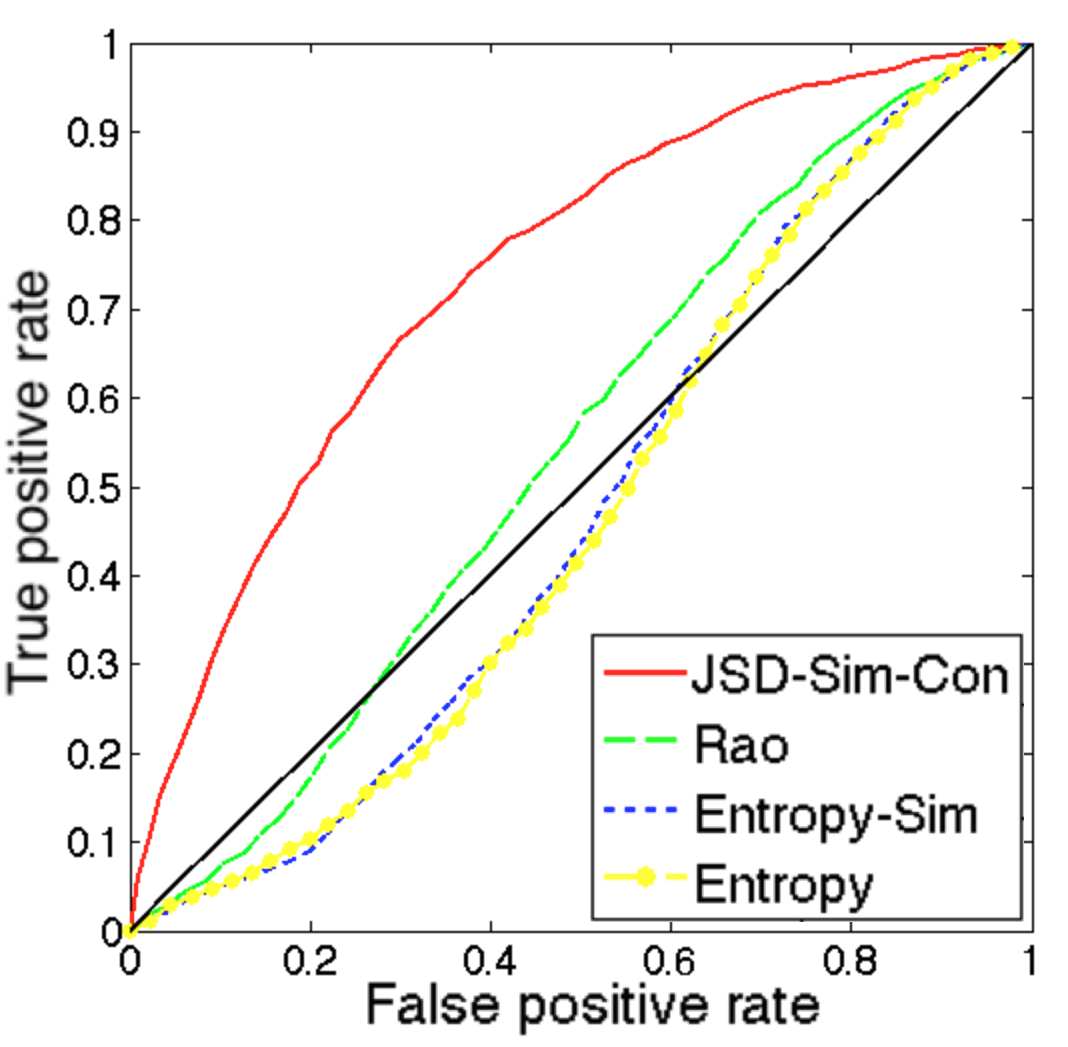
\includegraphics[width=36mm]{../nips-ml-nlp/figures/phonecases-comparison-kopia.png}
               \caption{eBay (baseline)}
                \label{fig:phonecases-comparison}
        \end{subfigure}%\qquad
              ~ %add desired spacing between images, e. g. ~, \quad, \qquad, \hfill etc.
          %(or a blank line to force the subfigure onto a new line)
        \begin{subfigure}[b]{0.24\textwidth}
                \centering
                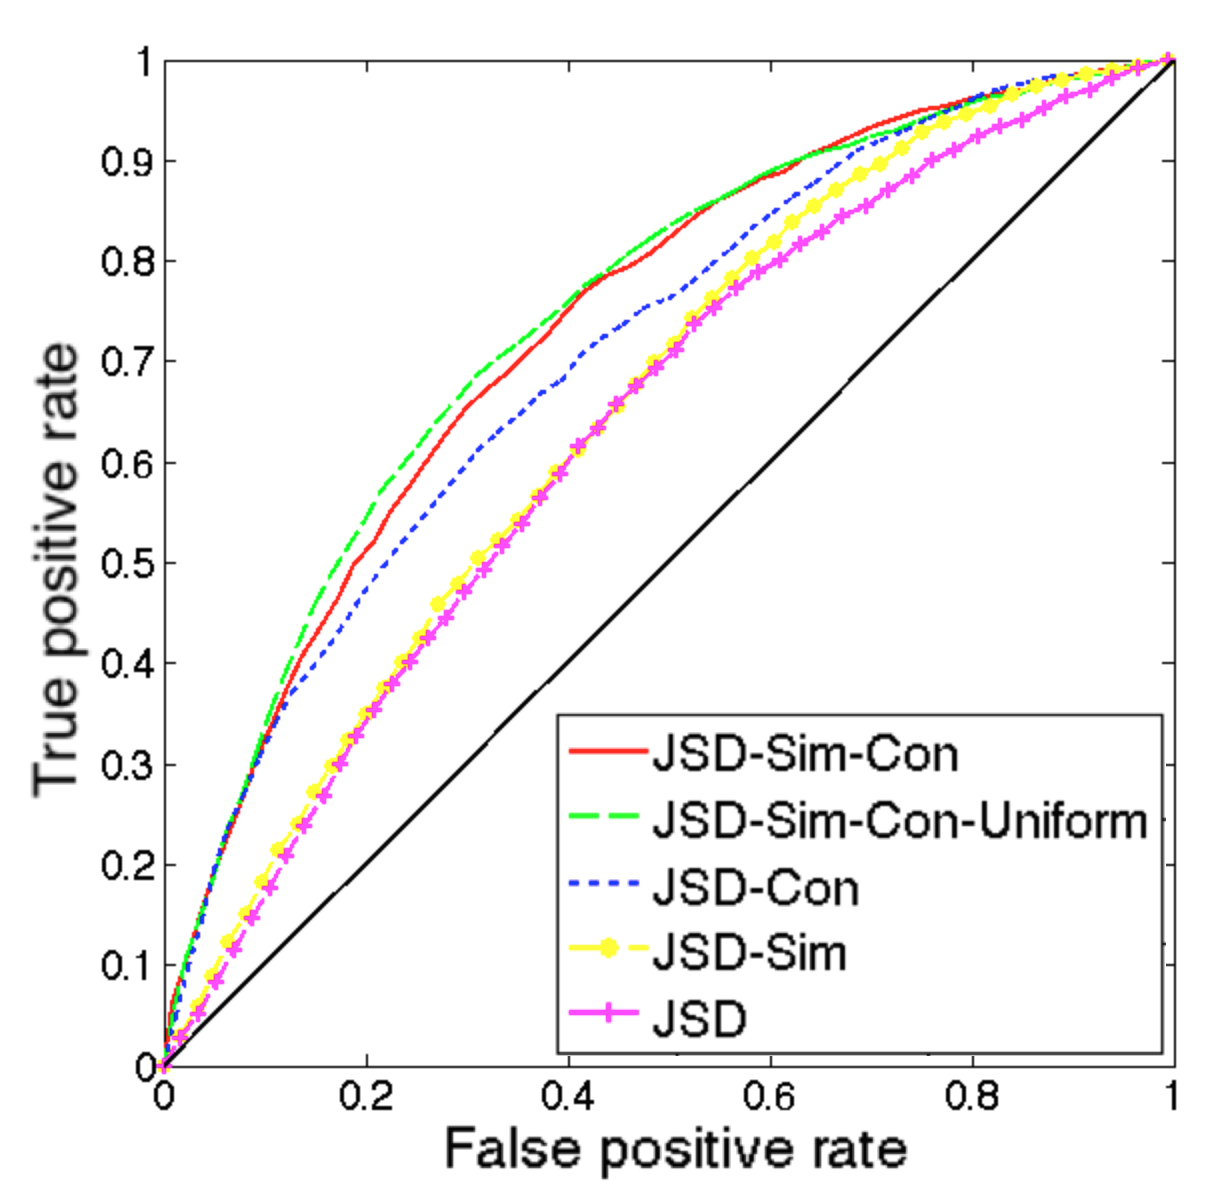
\includegraphics[width=36mm]{../nips-ml-nlp/figures/phonecases-breakdown-kopia.png}
                \caption{eBay (JSD)}
                \label{fig:phonecases-breakdown}
        \end{subfigure}\nobreak
              ~ %add desired spacing between images, e. g. ~, \quad, \qquad, \hfill etc.
          %(or a blank line to force the subfigure onto a new line)
        \begin{subfigure}[b]{0.24\textwidth}
                \centering
                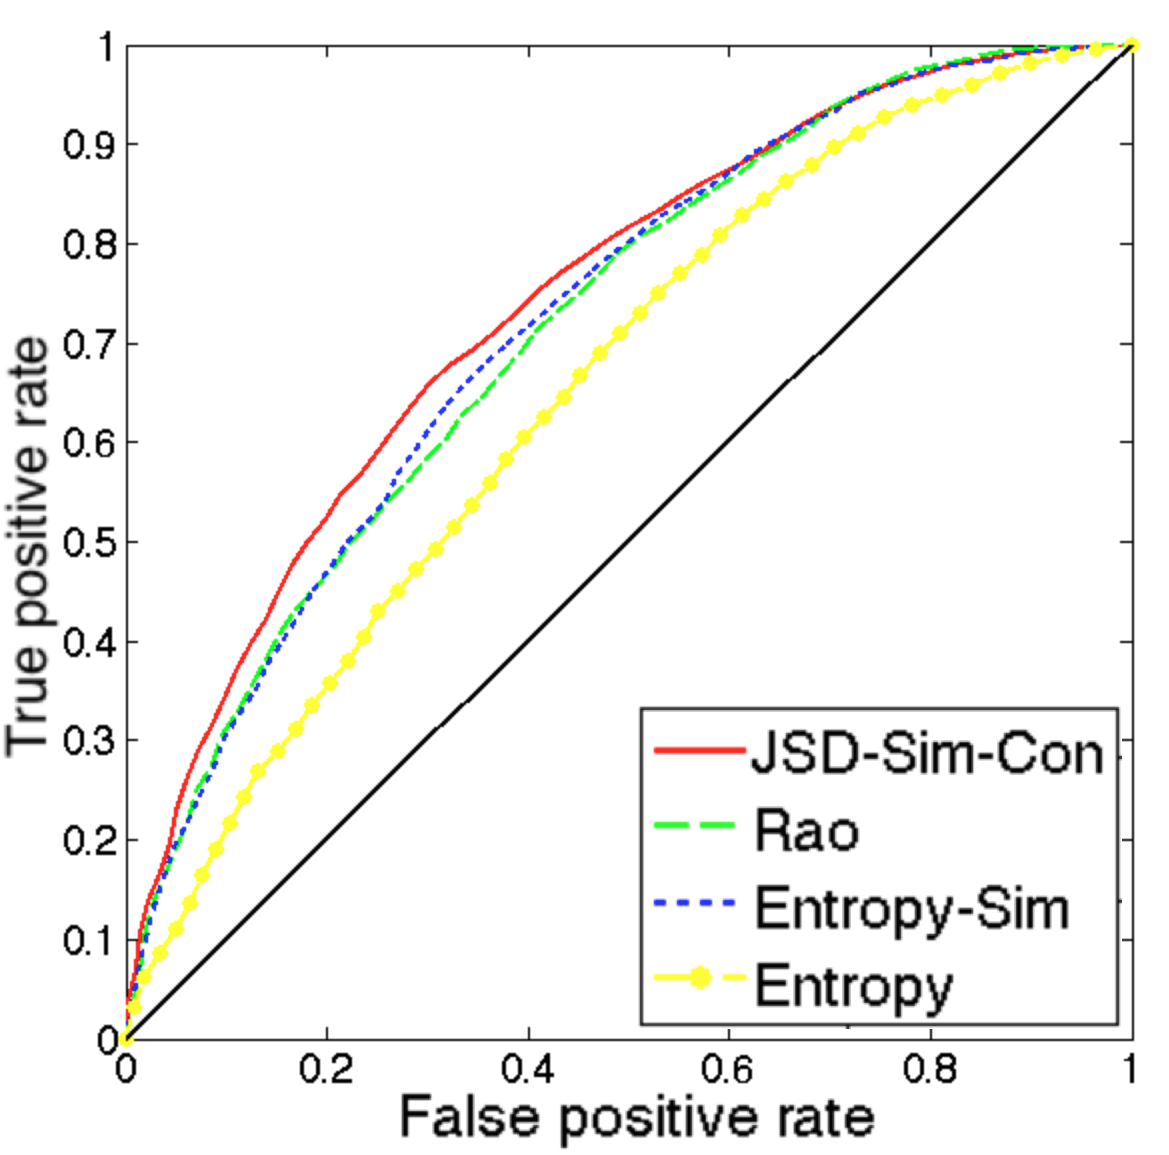
\includegraphics[width=36mm]{../nips-ml-nlp/figures/nsf-comparison-kopia.png}
                \caption{NSF (baseline)}
                \label{fig:nsf-comparison}
        \end{subfigure}%\qquad
        ~ %add desired spacing between images, e. g. ~, \quad, \qquad, \hfill etc.
          %(or a blank line to force the subfigure onto a new line)
        \begin{subfigure}[b]{0.24\textwidth}
        	        \centering
                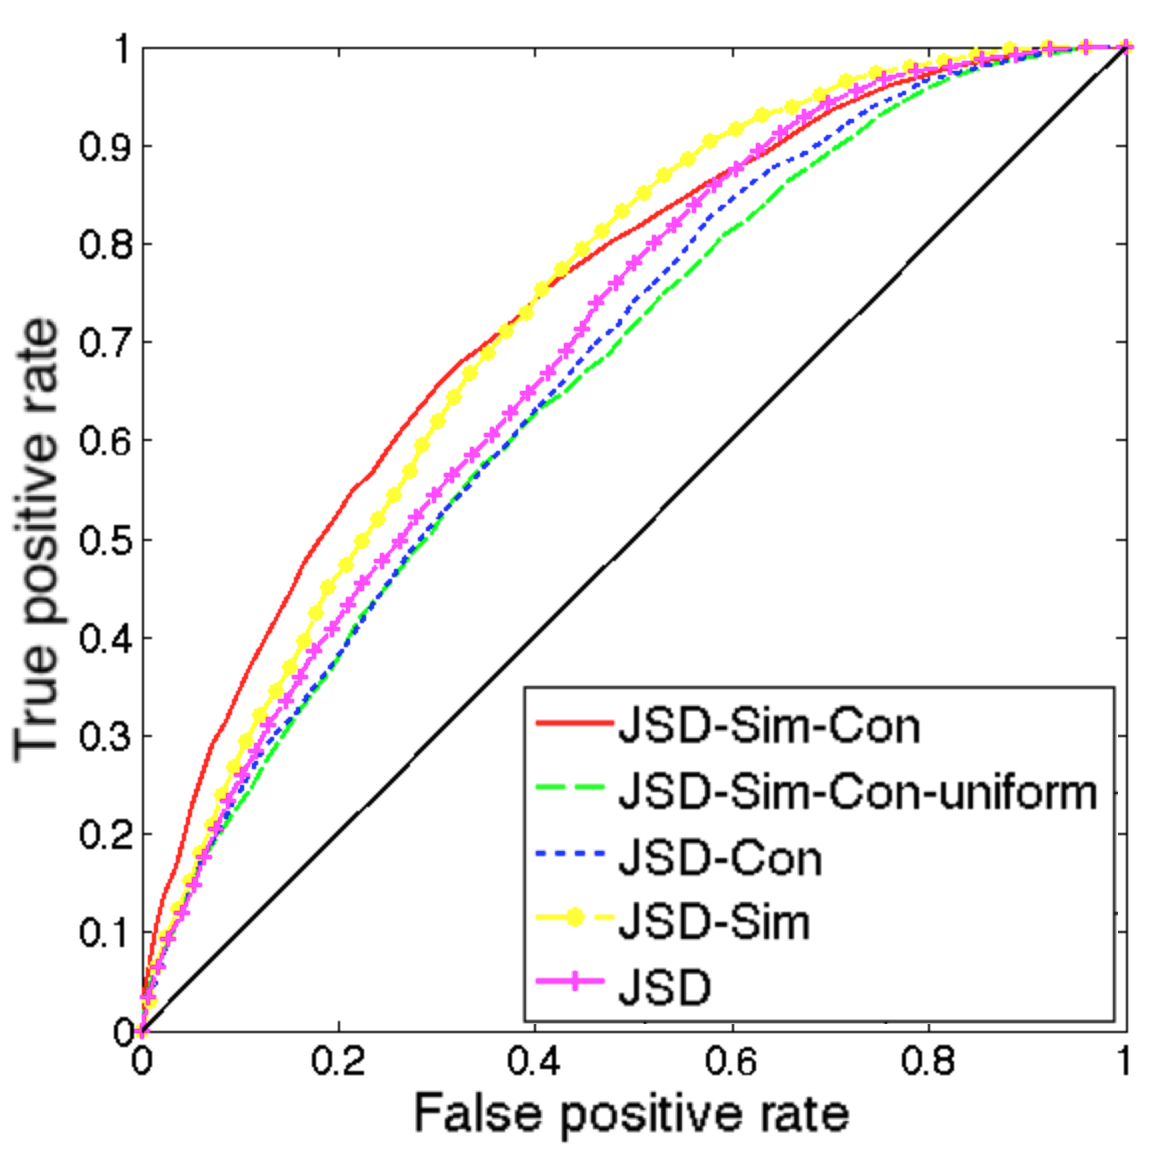
\includegraphics[width=36mm]{../nips-ml-nlp/figures/nsf-breakdown-kopia.png}
               \caption{NSF (JSD)}
                \label{fig:nsf-breakdown}
        \end{subfigure}
       \caption{ROC curves presenting the results of experiments on
         the eBay dataset (a,b) and NSF proposal dataset (c,d). The
         comparison plots (a,c) show the results for our approach (JSD-Sim-Con)
         against other methods, while the plots (b,d)
         show different variations of our approach. }\label{fig:roc-curves}
\end{figure}


\begin{table}[t]
\caption{Classification results for the eBay dataset.}
\label{tab:classification-results}
\vspace{-4mm}
\begin{center}
\begin{tabular}{|l|c|c|c|c|}
\hline
&Precision & Recall & F1 & Accuracy
\\ \hline 
JSD Features         &$\mathbf{0.714}\pm 0.015$&$0.597\pm 0.016$&$0.650\pm
0.014$& $\mathbf{0.8828}\pm 0.0045$\\
RAE             &$0.676\pm 0.005$&$\mathbf{0.666}\pm 0.030$&$\mathbf{0.671}\pm
0.013$&$0.8809\pm 0.0020$ \\
SVD Features             &$0.676\pm 0.008$&$0.633\pm 0.017$&$0.654\pm
0.010$&$0.8778\pm 0.0027$\\
\hline
\end{tabular}
\end{center}
\end{table}

\bibliographystyle{plain}
\bibliography{theory}


\end{document}